\chapter{System-Software}

\section{System-Struktur}
Die System-Struktur ist auf der Abbildung \ref{fig:system-software-system-struktur} ersichtlich. Das Dateisystem ist für gewöhnlich hierarchisch gegliedert. Speziell: Auf Linux-Systemen werden Peripherie-Geräte als Files behandelt, unter /dev für device.

\begin{figure}[h!]
\centering
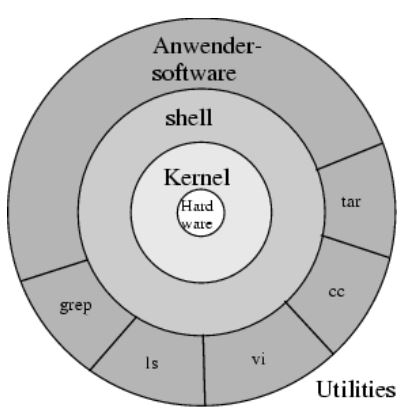
\includegraphics[width=0.4\linewidth]{fig/system-software-system-struktur}
\caption{System-Struktur}
\label{fig:system-software-system-struktur}
\end{figure}

\begin{figure}[h!]
	\centering
	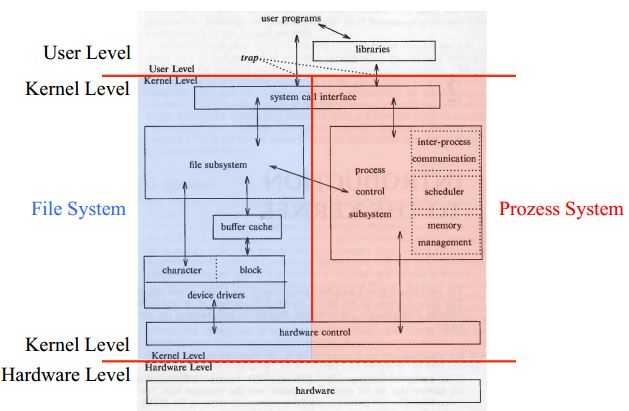
\includegraphics[width=0.7\linewidth]{fig/system-software-systemkern}
	\caption{System-Kern}
	\label{fig:system-software-systemkern}
\end{figure}

\subsection{Interrupt-Prioriäten}
\begin{enumerate}
	\item Maschinenfehler (höchste)
	\item Zeitgeber
	\item Disk
	\item Netzwerk
	\item Terminals
	\item Software-Interrupts (niedrigste)
\end{enumerate}

\subsection{Prozess-Elemente}
Ein Prozess kann einzigartig identifiziert werden durch: Identifier (PID), State, Priority, Program Counter, Memory Pointers, Context data, I/O Status infos, accounting infos.

Ein Programm ist eine ausführbare Datei. Ein Prozess ist ein in Ausführung befindendes Programm.

\paragraph{Prozess-Kontrol-Block} Enthält alle Prozess-Elemente. Wenn man alle Elemente eines Prozess hat, kann man diesen quasi schlafen legen (unterbrechen) und später wieder ausführen. Für den Prozess selber ist es so, als wäre er nie unterbrochen worden. Erzeugt und verwaltet durch das OS.

\paragraph{Prozess-Status} Trace (verfolgt): Zeichnet die Instruktionen eines Prozess auf und kann in aufgrund dessen charakterisieren. Dispatcher (verteilt): Kleines Programm, welches die Prozesse auf dem Prozesser wechselt.

\paragraph{Queuing Modell} Das OS arbeitet intern mit Queues um die Prozesse zu verwalten. Die unterschiedlichen Prozess Status sind als Queues implementiert (Ready-Queue, Blocked-Queue, usw.). Und sobald wieder einer an den Prozesser darf, kann er aus der Ready-Queue genommen werden.

\paragraph{OS Control Tables} Für die einzelnen Ressourcen werden Tabellen unterhalten, wie Memory Tables, I/O Tables, File Tables, Prozess Tables.

\paragraph{Process Control Structures}
Um einen Prozess zu verwalten, muss das OS folgendes wissen:
\begin{description}
	\item[Prozess Location] Ein oder mehrere Programme zum Ausführen. Genug Memory um Programm und dessen Daten zu halten. Einen Stack!
	\item[Prozess Attributes] Als Prozess Image wird die Sammlung der Programme, Daten, Stack und Attributen bezeichnet. Jeder Prozess hat zudem diverse Attribute, welche sich pro OS unterscheiden können.
\end{description}

\newpage
\subsubsection{Prozess-Image}
\begin{figure}[h!]
\centering
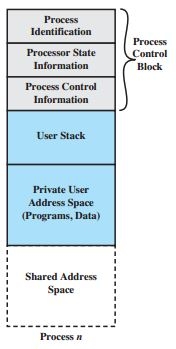
\includegraphics[width=0.2\linewidth]{fig/system-software-prozess-image}
\caption{Prozess-Image}
\label{fig:system-software-prozess-image}
\end{figure}

\paragraph{Virtueller zur physikalischem Adress-Übersetzung}
Wird mittels MMU (Memory Management Unit) gelöst. Mappt physical pages to virtual pages. \\

\subsubsection{Prozess wechsel}
\begin{figure}[h!]
\centering
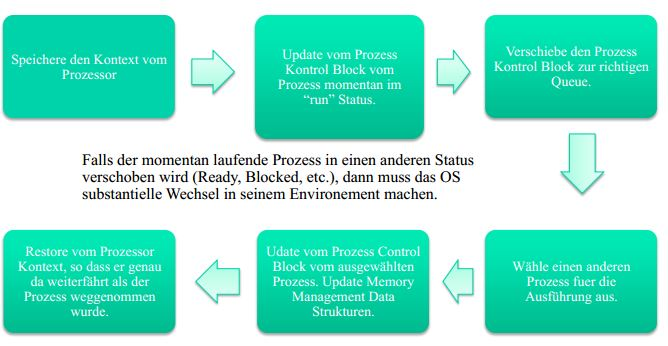
\includegraphics[width=0.7\linewidth]{fig/system-software-prozess-wechsel}
\caption{Prozess-Wechsel Vorgang}
\label{fig:system-software-prozess-wechsel}
\end{figure}

\newpage
\subsubsection{State-Engine Processes in UNIX}
\begin{figure}[h!]
\centering
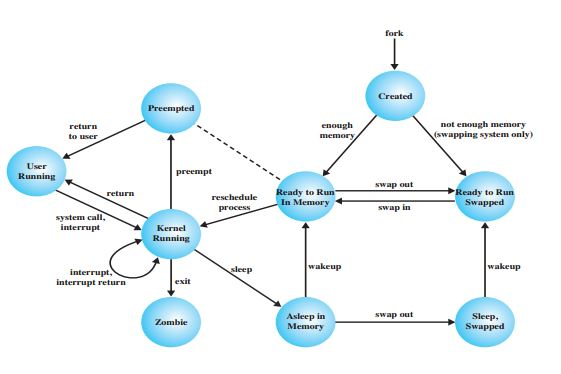
\includegraphics[width=0.9\linewidth]{fig/system-software-state-engine-processes-unix}
\caption{State Engine Processes in UNIX}
\label{fig:system-software-state-engine-processes-unix}
\end{figure}


\section{Prozess erzeugen}
Prozess wird mittels Kernel system call \texttt{fork()} erueigt. Anschliessend werden folgende Schritte durchgegangen:
\begin{enumerate}
	\item Freien Platz in der Prozesstabelle reservieren
	\item PID für den Prozess vergeben (der neue Prozess ist zwangsweise ein Child-Prozess)
	\item Kopiere Parent-Prozess Image mit Ausnahme des ''gesharten'' Memory
	\item Zähler für die Files inkrementieren. Um aufzuzeigen, dass ein zusätzlicher Prozess nun auf die Files zugreift.
	\item Prozess in ready-to-run Queue einfügen
	\item PID vom Child-Prozess zum Parent-Prozess übergeben (return value of \texttt{fork()}). Der Child-Prozess bekommt den Wert 0.
\end{enumerate}

Nachdem der Prozess erzeugt ist, ist er wie jeder andere Prozess. Kann also auch dispatched werden.

\section{Traps}
Es gibt diverse Varianten um Prozesse während der Ausführung zu unterbrechen:
\begin{description}
	\item[Interrupt] Externes Event tritt ein, bei der Ausführung einer Instruktion. Damit können asynchrone Events gehandelt werden.
	\item[Trap] Verknüpft mit der Ausführung der aktuellen Instruktion. Handling eines Fehlers oder einer Ausnahme.
	\item[Supervisor call] Expliziter Request. Aufruf einer OS-Funktion.
\end{description}

Speziell zu erwähnen ist, dass wir zwischen Benutzer-Stack (user) und System-Stack (kernel) unterscheiden.

\subsection{System-Calls}
System-Calls sind die Schnittstelle zwischen dem Betriebssystem und dem Benutzerprogramm. Wir stellen uns eine Single-Core Maschine vor. Der aktuelle Prozess arbeitet gerade im Benutzermodus. Nun will er einen Systemaufruf (lesen einer Datei) machen. Dazu muss eine Unterbrechung oder eine spezielle Systemaufruf-Anweisung durchführen. Dadurch wird die Kontrolle an das BS übergeben. Der Kern führt den Systemcall aus und gibt nach Abschluss die Kontrolle wieder zurück. Ein Systemcall ist wie eine gewöhnliche Prozedur, jedoch können nur Systemcalls in den Kern eintreten, gewöhnliche nicht.

In der Abbildung \ref{fig:system-software-ablauf-c-read} wird ein Trap ausgeführt in Schritt 6. Da wechselt das Programm vom Benutzermodus in den Kernelmodus. Im Schritt 9 wird kein Trap mehr durchgeführt, das zurückspringen passiert wie bei einer normalen Funktion.

Der SystemCall kann den Aufrufer auch weiterhin blockieren. Wenn das Anwenderprogramm nämlich Input von der Tastatur möchte (mittels SystemCall) und nichts kommt, dann blockiert das BS und lässt andere Prozesse arbeiten.

\begin{figure}[h!]
\centering
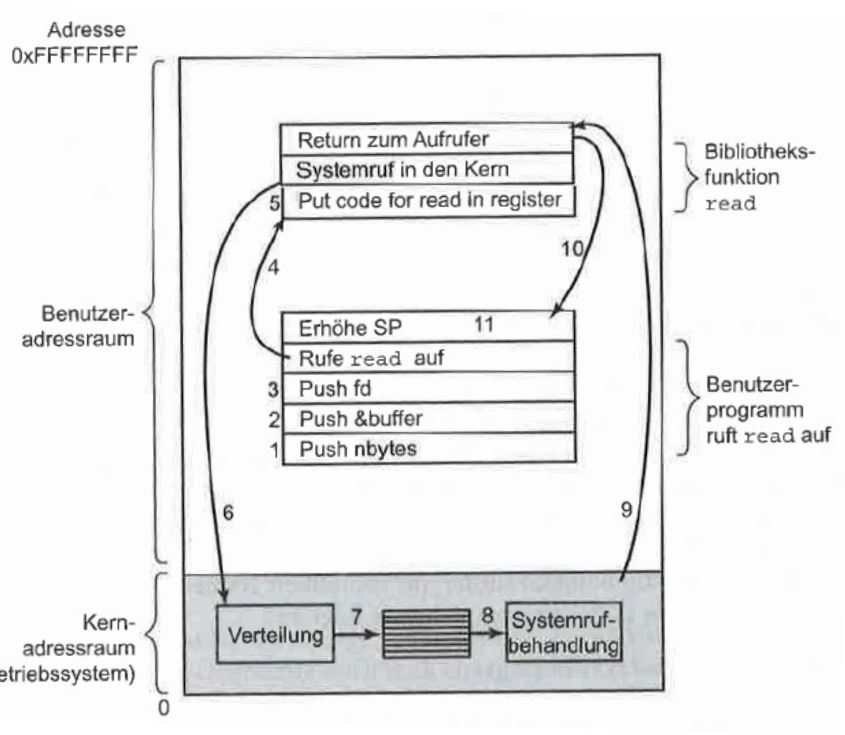
\includegraphics[width=0.6\linewidth]{fig/system-software-ablauf-c-read}
\caption{System-Call am Beispiel von C read}
\label{fig:system-software-ablauf-c-read}
\end{figure}


\section{Prozess-Kontext}
Wir unterscheiden zwischen drei Bereichen:
\begin{description}
	\item[Benutzer Kontext] Zugewiesener Adressraum und Daten.
	\item[Hardware Kontext] Multitasking relevant. Inhalte der CPU Register, Seitentabellen etc.
	\item[System Kontext] OS Sicht. PID, geöffnete Dateien, Info Eltern und Kind Prozesse, Prioritäten etc. 
\end{description}

\paragraph{File-Deskriptoren}
Jedes geöffnete File erhält eine ID. Jeder Prozess hat seine eigene File Deskriptoren Tabelle, welche eine Sammlung von Pointer ist zu den I/O Streams.

Standard File Deskriptoren: Keyboard to Program über 0 stdin. Keyboard to Display über 1 stdout oder 2 stderr.

Diese Standard-Kanäle können umgebogen werden. Mittels >, 2>, 1>\&2, \&>/dev/null

\section{Threads}
Die Idee kennen wir. Leichtgewichtige Threads vs. schwergewichtige Prozesse. Unter einem einzigen Prozess können mehrere Threads laufen. Im Gegensatz zu Prozessen ist die Erzeugung, Beendigung und Wechsel zwischen Threads um einiges schneller. Auch die Kommunikation ist auf natürlich weise mit dem gemeinsamen Prozess Kontext gegeben.

\begin{figure}[h!]
\centering
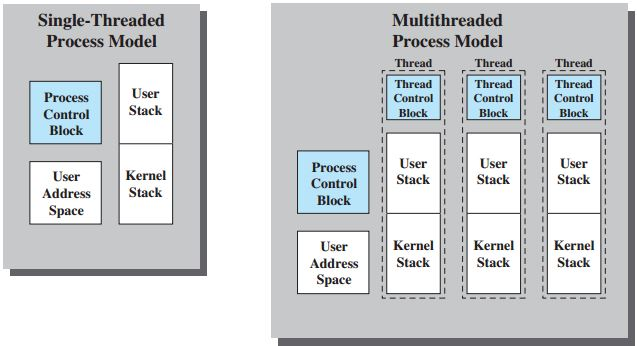
\includegraphics[width=0.7\linewidth]{fig/system-software-single-threaded-vs-muli-threaded}
\caption{Single Threaded vs. Multi-Threaded}
\label{fig:system-software-single-threaded-vs-muli-threaded}
\end{figure}

\subsection{Thread-Kontext}
Ein Prozess besteht aus mind. 1 Thread. Threads vom gleichen Prozess teilen sich Codesegmente, Datensegmente und Dateideskriptoren. Jeder Thread hat seinen Stack und seinen Code Pointer.

\subsection{Thread-Arten}
\begin{description}
	\item[User Level Threads ULT]
	Thread Mgmt. in der Applikation. Der Kern hat keine Kentniss über die Existenz von Prozessen. Arbeiten komplett im User Space. Müssen Kontrolle von sich aus abgegeben. Neigen mehr zu kooperativem als zu preemptiven Scheduling. Implementieren manchmal das Scheduling selber (z.B. frühere Versionen von Java.).
	Dafür gibt es ein paar Vorteile: Thread Wechsel verlangt keinen Kernel Modus, Scheduling applikationspezifisch, ULTs laufen auf jedem OS.
	\item[Kernel Level Threads KLT]
	Thread Mgmt. vom Kern. Windows verfolgt diesen Ansatz. Der Kern kann mehrere Threads vom gleichen Prozess auf mehrere Prozessoren verteilen (Scheduling). Wenn ein Thread blockiert ist, kann ein Thread vom gleichen Prozess berücksichtigt werden. Kern Prozeduren können multithreaded ausgeführt werden.
\end{description}

\subsection{Kombinierter Ansatz}
Oft kommt wohl eine Kombination zum Zug. Thread Erzeugung und generelles Thread Management wird von der Applikation gemacht. Der Rest ist Kernel Sache. Solaris ist ein Vertreter.

\subsection{Zwei Level Thread Modell}
Verlegen von Threads ist schnell. Erzeugen/Löschen sind eher kostspielige Operationen. Daher wurde eine weitere Schicht eingeführt, die sogeannten LWP (lightweigh process). Die User-Threads werden den LWPs zugeführt. Nur die Threads auf den LWPs sind aktiv. Dabei beinhaltet die LWPs die Kernel Level Threads, welche für die Kernel Level Tasks verwendet werden.

Das OS verwendet schlussendlich wirklich nur die Kernel Level Threads. 

\begin{figure}[h!]
\centering
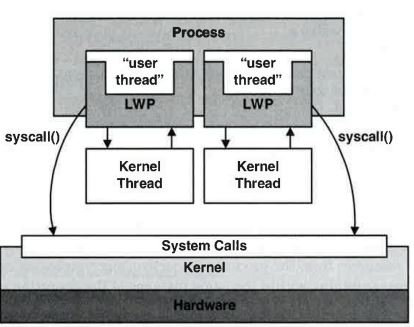
\includegraphics[width=0.7\linewidth]{fig/system-software-aufbau-2-level-threading}
\caption{Aufbau Zwei Level Threading}
\label{fig:system-software-aufbau-2-level-threading}
\end{figure}

\subsection{Windows-Prozesse}
Prozesse existieren als Objekte. Werden als neue oder als Kopie bestehender Prozesse erzeugt. Kann pro Prozess auch mehrere Threads beinhalten. Sowohl Prozesse wie auch Threads haben eingebaute Synchronisierungs-Mechanismen.